% !TeX program = pdflatex
% !TeX encoding = utf8
% !TeX spellcheck = russian_english
% !BIB program = biber


\documentclass{LabWorkEng}
\usepackage[type=none]{fgruler}
\addbibresource{\jobname.bib}

\tikzset{
	magarrow/.pic = {
		\fill [blue] (0,-0.25) rectangle (0.25,0.25);
	}
}

\newcolumntype{C}{>{\centering\arraybackslash}p{5em}}
\title{Study of the laws of rotational motion on the example of Oberbek pendulum}
\work{2}

\abstract{study of the rotational motion of the Oberbeck pendulum, depending on the applied torque moment and the moment of inertia of the pendulum.}



\keywords{Rotational motion of bodies, angular acceleration, torque, moment of inertia}

\apparatus{Oberbeck pendulum; set of loads; stopwatch; scale ruler, scales.}

\begin{document}
\writedatatofile{\jobname}
\maketitle

\nocite{IrodovMechanics, BerkeleyMechanics, FLF1, Holyday}
\printbibliography

\section{Theoretibal background}

The rotational motion is an example of a simple mechanical motion. To describe the rotational motion, the following categories are used: the moment of inertia of the body and the moment of force (also known as torque). For a single material point, the moment of inertia relative to the axis of rotation is called the product of mass on the square of the distance to this axis. The moment of inertia $J$ of the system of material points with mass $m_i$ is the sum of the moments of individual points.
\begin{equation}\label{1}
	J = \sum\limits_i {{m_i}r_i^2}
\end{equation}
Torque $\vec M$ relative to the point is called the vector multiplication of radius-vector $\vec r$  from the point  to the place of application of force on the active force:
\begin{equation}\label{2}
	\vec M = \vec r \times \vec F
\end{equation}
Module (absolute value) of the moment of force:
\begin{equation}\label{2'}
	 M = r \cdot F \cdot \sin\alpha
\end{equation}
where $\alpha$ -- angle between the vectors $\vec F$  and $\vec r$. $R\sin\alpha$ -- this is shoulder of force, that equals to length of the perpendicular, carried out from the beginning of the radius vector $\vec r$  to the line of force.
The torque relative to the rotation axis is a scalar value equal to the projection of the vector moment of force  on this axis relatively to any point on the axis. 


The motion of a body with a moment of inertia $J$, rotating at an angular velocity $\omega$ around the stationary axis, is described by the following equation:
\begin{equation}\label{3}
	\frac{d}{{dt}}\left( {J\omega } \right) = M
\end{equation}
where $M$ -- moment of external forces relative to the axis rotation. When the solid is rotated its moment of inertia does not depend on time and equation~\eqref{3} is simplified:
\begin{equation}\label{4}
	 J\frac{{d\omega }}{{dt}} = M
\end{equation}
The equation~\eqref{4} is similar to the Newton equation $ma=F$, which describes the motion of a material point. The moment of force $M$ plays the role of force $F$, the moment of inertia $J$ plays the role of mass $m$, the angular acceleration $\beta = \frac{d\omega}{dt}$ is analogous to linear acceleration $a = \frac{dv}{dt}$.

\noindent%
\begin{Think}
	\begin{enumerate}
	\item Why does the bicycle wheel have many knitting needles? What would be if the knitting needles were only two?
	\item Why, when they throw a stone, they try to take their hand as far away from the body as possible?
\end{enumerate}
\end{Think}

\section{Theoretical basis of the experiment}

The Oberbeck pendulum is schematically represented in Fig.~\ref{pic}. Four needles, fixed on the sleeve, form one another with straight angles. The common axis passes through the sleeve and two pulleys with radii $r_1$ and $r_2$. The axis is secured in the needle shafts so that the entire system can rotate freely around the horizontal axis. The moment of inertia of the device can be changed by moving the loads $m$ along the needles.

A thin thread is wound on one of the pulleys of the pendulum. The weight of the known mass is tied to the thread. (The set includes bodies of different masses). Rotating moment is formed by the force of the thread tension $T$:
\begin{equation}\label{5}
	M_i = r_iT,
\end{equation}
where $i = 1, 2$.

The force T can be found from the mass equation of body with mass $m_0$:
\begin{equation}\label{6}
	m_0g - T = m_0a
\end{equation}
Acceleration a is proportional to angular acceleration $\beta$:
\begin{equation}\label{7}
	a_i = \beta r_i,
\end{equation}
where $i = 1, 2$ and is determined experimentally. Indeed, by measuring the time $t$, for which the body from the state of rest decreases by distance $h$, we find a by the formula
\begin{equation}\label{8}
	a = \frac{2h}{t^2}.
\end{equation} 

The system of equations \eqref{5} -- \eqref{8} allows determining the moment of inertia of the pendulum and checking the general equation of dynamics~\eqref{4} provided that the moment of friction of the Mfric relative to the pendulum axis is much smaller than the moment of tensile force of the thread $T$. 

In fact, the moment of friction of the Mfric can be quite large and lead to distortion of measurement results. At first sight, it seems that reducing the role of friction forces can be due to an increase in the mass of solid $m_0$. But such a view is false because
\begin{enumerate}
	\item an increase in the mass $m_0$  leads to an increase in the pressure of the pendulum on the axis and, thus, to increase the frictional forces;
	\item an increase in $m_0$ leads to a decrease in the time of the fall of the weight, which reduces the accuracy of the measurement of time.
\end{enumerate}


In the proposed installation, the friction forces are reduced due to the use of needle bearings for attaching the pendulum axis. In spite of this, it is impossible to completely prevent the influence of friction force and this should be taken into account when processing the results of the experiment.

When processing the results of an experiment it is convenient to rewrite the equation~\eqref{4} in such a way that it contains the moment of frictional forces in explicit form:
\begin{equation}\label{4'}
	J\frac{d\omega}{dt} = M - {M_{fric}}.
\end{equation}

The moment of inertia of the system is determined by the formula:
\begin{equation}\label{9}
	J = {J_0} + 4m{R^2}
\end{equation}
where $J_0$ -- moment of inertia of the system without loads, $R$ -- distance from the axis of rotation to the center of mass of loads.
%, $J_B$ -- moment of inertia of one load relative to the axis passing through its center of mass parallel to the axis of rotation. We propose to derive this formula yourself.

\begin{figure}[!t]
	\centering
	\begin{subfigure}[t]{0.4\linewidth}\centering
		\begin{picbox}	
			\begin{tikzpicture}
			\tikzstyle{ground}=[fill,pattern=north east lines,draw=none,minimum width=0.75cm,minimum height=0.3cm]
			\node (wall1) [ground, minimum width=3cm] {};
			\draw (wall1.north west) -- (wall1.north east);
			\fill[gray!50] (-0.25,0.3) rectangle (0.25,10);
			\foreach \i in {1,2,3,4} {\draw[thick] (0,10) --  pic[pos=0.7, rotate = \i*90 + 45] {magarrow} +(\i*90 + 45:4);}
			\draw[ultra thick, fill=white] (0.0,10) circle (1);
			%\node[above] at (0.0,11) {$1$};
			\draw[fill=gray] (0.0,10) circle (0.1);
			\draw (1,10) -- (1,4);
			\draw[thick, fill=gray] (0.7,4) rectangle node[text = white] {} +(0.6,-1);
			\fill[gray, draw=black] (0.2,8) rectangle +(1.3,-0.1) node[below, text = black] {$2$} ;
			\fill[gray, draw=black] (0.2,2) rectangle +(1.3,-0.1) node[below, text = black] {$3$};
			\fill[gray!50, draw = black] (-1,0.3) rectangle +(2,1);
			\fill[red] (-0.9,1) rectangle +(0.3,0.1);
			\fill[black] (-0.9,0.8) rectangle +(0.3,0.1);
			\fill[black] (-0.9,0.6) rectangle +(0.3,0.1);
			\draw[fill=white] (-0.5,0.6) rectangle node[text = red] {time} +(1.3,0.5);
			\fill[black] (-0.9,0.15) rectangle +(0.3,0.15);
			\fill[black] (0.6,0.15) rectangle +(0.3,0.15);
			\node at (0.1,5) {\fgrulerdefnum{}\fgrulercaptioncm{}\ruler{upleft}{7cm}};
			\end{tikzpicture}
		\end{picbox}
		\subcaption{}
		%\label{Atwood_machine}
	\end{subfigure}
	\begin{subfigure}[t]{0.4\linewidth}\centering
		\begin{picbox}	
			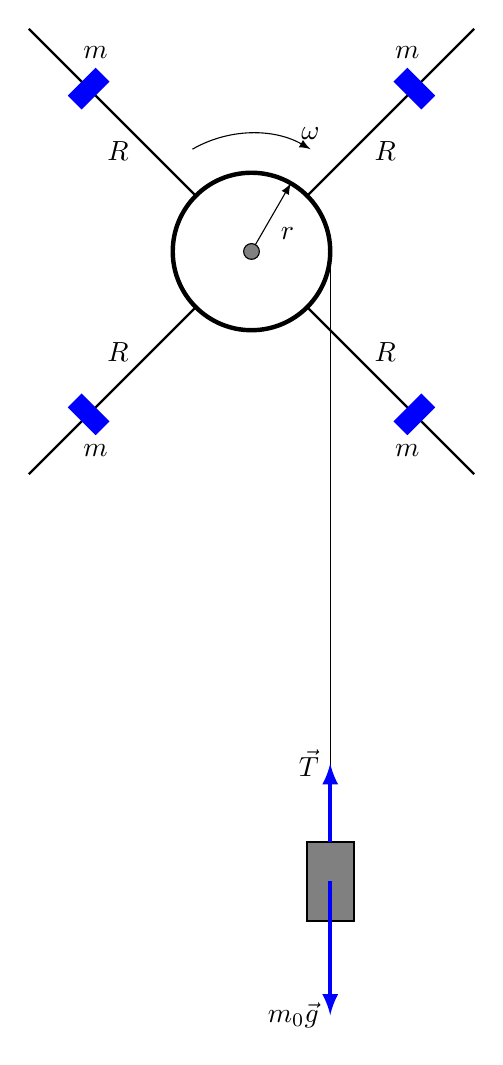
\begin{tikzpicture}
			\draw[-latex] (0,10) +(120:1.5) arc(120:60:1.5) node[above] {$\omega$};
			\foreach \i in {1,2,3,4} {\draw[thick] (0,10) --  pic[pos=0.7, rotate = \i*90 + 45] {magarrow} coordinate[pos =0.7] (A\i) coordinate[pos = 0.6] (B\i) +(\i*90 + 45:4);}
			\node[above=10pt] at (A1) {$m$};
			\node[above=10pt] at (A4) {$m$};
			\node[below=10pt] at (A2) {$m$};
			\node[below=10pt] at (A3) {$m$};
			
			\node[below=5pt] at (B1) {$R$};
			\node[below=5pt] at (B4) {$R$};
			\node[above=5pt] at (B2) {$R$};
			\node[above=5pt] at (B3) {$R$};
			
			\draw[ultra thick, fill=white] (0.0,10) circle (1);
			\draw[-latex] (0,10) -- node[below right] {$r$} +(60:1) ;
			%\node[above] at (0.0,11) {$1$};
			\draw[fill=gray] (0.0,10) circle (0.1);
			\draw (1,10) -- (1,3);
			\draw[thick, fill=gray] (0.7,2.5) rectangle node[text = white] {} +(0.6,-1);
			\draw[ultra thick, blue, -latex] (1,2.5) -- +(0,1) node[left, text = black] {$\vec T$};
			\draw[ultra thick, blue, -latex] (1,2) -- +(0,-1.7) node[left, text = black] {$m_0\vec g$};
			\end{tikzpicture}
		\end{picbox}
		\subcaption{}
		%\label{Forces}
	\end{subfigure}
	\caption{}
	\label{pic}
\end{figure}

\section{Experimental details}

Time of movement of the body is measured by an electronic stopwatch, which is activated and deactivated by signals from photo sensors. The beginning and end of the motion of the body is recorded by its passage of the optical axis of the photodetector, so before the experiment begins, the lower end of the body should be located directly above the optical axis of the upper photosensor. 

The photosensors and the digital display are activated when the device is switched on. This also includes a friction brake that holds the pendulum in a given position. The brake is deactivated if you press the \tcbox{\sc{Start}} button and hold it in the pressed state.

The height of fall is determined by the scale applied to the riser, by the difference in positions of the optical axes of the upper and lower photosensors.

\section{Tasks}
\begin{enumerate}
	\item Investigate the rotational motion of the pendulum under the influence of various weights at a constant moment of inertia of the system.
	\begin{enumerate}
		\item\label{first} Place the loads $m$ at a certain distance $R$ from the axis of rotation and achieve the indifferent equilibrium of the pendulum. Measure and record the distance $R$.
		\item\label{second} Conduct an experiment with the weight of the mass $m_0$, measuring the time of fall of the weight. The experiment should be repeated $8-10$ times, and then $t$ should be averaged.
		\item\label{third} Repeat the experiment of point~\ref{second} on both pulleys for 3-4 different values of $m_0$.
	\end{enumerate}
	\item Repeat measurements~\ref{second}, \ref{third} for $3-4$ different values of the moment of inertia of the system.
	\item Repeat measurements~\ref{second} for $3-4$ different values of the masses $m_0$ for the system without loads $m$.
%	\item Make the necessary measurements to determine your own moment of inertia of bodies $J_B$.
\end{enumerate}

\section{Processing the results of the experiment}

\begin{enumerate}
	\item Using measurements~\ref{second} and \ref{third} find the angular acceleration $\beta$ and the torque moment $M$ corresponding to the movement of each of the bodies on both pulleys for all values of the moment of inertia of the system $J$. Determine the error.
	\item For each value of $R$, graphically represent the dependence of the angular acceleration $\beta$ on the rotating torque $M$. Determine the moments of inertia of the system $J$ and moments of the friction forces of the $M_{fric}$. What errors have these values?
	\item Compare the obtained values of $M_{fric}$. Does the value of Mfric depend on the moment of inertia of the system? Averaging the value of  $M_{fric}$.
	\item The results of the definition of $J$ at different values of $R$, are presented graphically as the dependence of  $J(R^2)$. Consider why it is proposed to build such a dependence. After processing the results, determine the moment of inertia of the system without loads $J_0$. How do the results of the experiment with formula~\eqref{9} consist? How does the magnitude of the experiment error with $J_B$? What are the possible sources of experimental errors?
\end{enumerate}

\section*{Control questions}

\begin{enumerate}
	\item Formulate the basic kinematic quantities of rotational motion and explain their physical meaning.
	\item Between what quantities does the basic law of dynamics of rotational motion establish a relationship?
	\item How is the magnitude and direction of the moments of forces (torque) determined? In what units is this value measured?
	\item What determines the moment of inertia, in what units is it measured? How to understand that the moment of inertia is an additive quantity? How it was used in the work?
%	\item Which of the values in this experiment should be measured with the highest accuracy?	
%	\item Why does the pendulum have exactly $4$ needles? What will change if you take only $2$ needles (or $6$ needles, for example)?	
%	\item How to find out if the pendulum is well balanced (is it really in indifferent the equilibrium)?
	\item Formulate and prove the parallel axes theorem.
\end{enumerate}

\end{document}